
% ===== Slide 3 =====
\section{Vector Equations}
\begin{frame}{Vector Equations}
  \centering
  \Large 1.3 Vector Equations

  \medskip
  % Optional Chinese subtitle from source: 向量方程
\end{frame}

% ===== Slide 4 =====
\begin{frame}{Recap}
  \begin{itemize}
    \item Augmented matrices lead us to consider rectangular arrays of
          numbers---matrices.
  \end{itemize}
  \[
    A=
    \begin{pmatrix}
      a_{11} & a_{12} & \cdots & a_{1n}\\
      a_{21} & a_{22} & \cdots & a_{2n}\\
      \vdots & \vdots & \ddots & \vdots\\
      a_{m1} & a_{m2} & \cdots & a_{mn}
    \end{pmatrix}.
  \]
\end{frame}

% ===== Slide 5 =====
\begin{frame}{Definition of matrix}
  \textbf{Definition:} A \alert{matrix} is a rectangular array of numbers.
  \[
    A=
    \begin{pmatrix}
      a_{11} & a_{12} & \cdots & a_{1n}\\
      a_{21} & a_{22} & \cdots & a_{2n}\\
      \vdots & \vdots & \ddots & \vdots\\
      a_{m1} & a_{m2} & \cdots & a_{mn}
    \end{pmatrix}.
  \]
  We say that $A$ has $m$ rows and $n$ columns. 
  
  The \alert{dimension}
  (or \alert{size}) of $A$ is $m\times n$ ($m$-by-$n$). 
  
  The element
  $a_{ij}$ is called the $(i,j)$th entry.
\end{frame}

% ===== Slide 6 =====
\begin{frame}{Special Matrix Shapes}
  An $m\times n$ matrix is a \alert{square matrix of order $n$} if $m=n$.
  % Chinese label in source: n阶方阵

  \medskip
  A $1\times n$ matrix is a \alert{\textbf{row matrix}} (or \textbf{row vector}):
  \[
    \begin{pmatrix}a_1&a_2&\cdots&a_n\end{pmatrix}.
  \]
  A $m\times1$ matrix is a \alert{column matrix} (or column vector):
  \[
    \begin{pmatrix}a_1\\a_2\\\vdots\\a_m\end{pmatrix}.
  \]

  \textbf{Abbreviation}: In \textbf{this} course we will often mention vectors. It is a column vector.

\end{frame}


% ===== Slide 7 =====
\begin{frame}{Vectors in $\mathbb{R}^2$}
  A vector with two entries has the form
  \[
    \mathbf{u}=\begin{bmatrix}u_1\\u_2\end{bmatrix},
    \qquad u_1,u_2\in\mathbb{R}.
  \]
  \begin{figure}
    
    \centering
    \textbf{ordered $2$-tuples}

  \end{figure}
  The set of all vectors with two entries is denoted by $\mathbb{R}^2$ (read ``R-two'').

  \medskip
  The $\mathbb{R}$ means the entries are real numbers, and the
  exponent $^2$ indicates that each vector contains two entries.
\end{frame}

% ===== Slide 8 =====
\begin{frame}{Geometric Description of $\mathbb{R}^2$}
  
    \begin{columns}
        \begin{column}{.4\linewidth}
        \begin{figure}
            \centering
            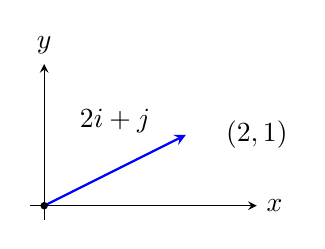
\begin{tikzpicture}[>=stealth,scale=0.9]
            \draw[->] (-0.2,0) -- (3,0) node[right] {$x$};
            \draw[->] (0,-0.2) -- (0,2) node[above] {$y$};
            \draw[->,thick,color=blue] (0,0) -- (2,1) ;
            \node at (3,1) {$(2,1)$};
            \node at (1,1.2) {$2i + j$};
            \fill (0,0) circle (1.5pt);
        \end{tikzpicture}
    \end{figure}
        
    \end{column}
    \begin{column}{.6\linewidth}
        \begin{tabular}{ccccc}
            \text{point}&$\Longleftrightarrow$&\text{vector} &$\Longleftrightarrow$&\text{column matrix}\\
            % \\
            (2,1)&&$2\mathbf{i}+\mathbf{j}$&&$\begin{pmatrix}2\\1\end{pmatrix}$\\
        \end{tabular}        

        % \[
        %     \text{point }(2,1)
        %     \quad\Longleftrightarrow\quad
        %     \text{vector }2\mathbf{i}+\mathbf{j}
        %     \quad\Longleftrightarrow\quad
        %     \text{column matrix }\begin{pmatrix}2\\1\end{pmatrix}.
        % \]
        Vector $\begin{bmatrix}x_1\\x_2\end{bmatrix}$ is the point $(x_1,x_2)$ in the plane. 
        
        $\mathbb{R}^2$ is the set of all points in the plane.
    \end{column}
\end{columns}


\end{frame}

% ===== Slide 9 =====
\begin{frame}{Vectors in $\mathbb{R}^3$ and $\mathbb{R}^n$}

{\color{blue}Vectors in $\mathbb{R}^3$ (vectors with 3 entries)}
  \[
    \mathbf{u}=\begin{bmatrix}u_1\\u_2\\u_3\end{bmatrix}
    \qquad\text{(an ordered $3$-tuple).}
  \]
{\color{blue}Vectors in $\mathbb{R}^n$ (vectors with $n$ entries)}
  \[
    \mathbf{u}=\begin{bmatrix}u_1\\u_2\\\vdots\\u_n\end{bmatrix}
    \qquad\text{(an ordered $n$-tuple).}
  \]
  written as $\mathbf{u}$ or $\vec{u}$.
\end{frame}

% ===== Slide 10 =====
\begin{frame}{The Zero Vector $\mathbf{0}$}

    {The \color{blue} zero vector $\mathbf{0}$}

  The vector whose entries are all zero.
  $\mathbf{0} = \begin{bmatrix}0\\0\\\vdots\\0\end{bmatrix}$\pause

  Well... appears useless right?
  
%   The number of entries in $\mathbf{0}$ will be clear from the context.
\end{frame}

% ===== Slide 11 =====
\begin{frame}{Vector Arithmetic: Addition}


    \begin{columns}
        \begin{column}{.4\linewidth}
        \begin{figure}
            \centering
            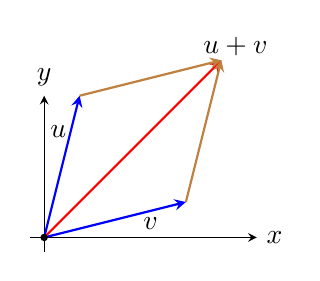
\begin{tikzpicture}[>=stealth,scale=0.9]
            \draw[->] (-0.2,0) -- (3,0) node[right] {$x$};
            \draw[->] (0,-0.2) -- (0,2) node[above] {$y$};
            \draw[->,thick,color=blue] (0,0) -- (0.5,2) ;
            \draw[->,thick,color=blue] (0,0) -- (2,0.5) ;
            \draw[->,thick,color=red] (0,0) -- (2.5,2.5) ;
            \draw[->,thick,color=brown] (0.5,2) -- (2.5,2.5) ;
            \draw[->,thick,color=brown] (2,0.5) -- (2.5,2.5) ;
            \node at (2.7,2.7) {$u+v$};
            \node at (0.2,1.5) {$u$};
            \node at (1.5,0.2) {$v$};
            \fill (0,0) circle (1.5pt);
        \end{tikzpicture}
    \end{figure}
        
    \end{column}
    \begin{column}{.6\linewidth}
        We can view each column as a vector.

        \begin{figure}
            \centering
            $u = \begin{bmatrix}0.5\\2\end{bmatrix}$

            $v = \begin{bmatrix}2\\0.5\end{bmatrix}$

            $u+v = \begin{bmatrix}2+0.5\\2+0.5\end{bmatrix}$
        \end{figure}

    \end{column}
\end{columns}
\end{frame}


% ===== Slide 11 =====
\begin{frame}{Vector Arithmetic: Addition}


    \begin{columns}
        \begin{column}{.4\linewidth}
        \begin{figure}
            \centering
            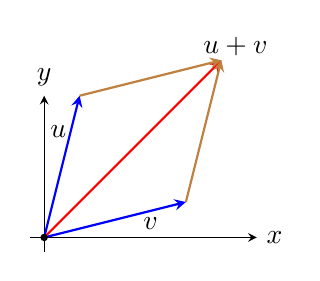
\begin{tikzpicture}[>=stealth,scale=0.9]
            \draw[->] (-0.2,0) -- (3,0) node[right] {$x$};
            \draw[->] (0,-0.2) -- (0,2) node[above] {$y$};
            \draw[->,thick,color=blue] (0,0) -- (0.5,2) ;
            \draw[->,thick,color=blue] (0,0) -- (2,0.5) ;
            \draw[->,thick,color=red] (0,0) -- (2.5,2.5) ;
            \draw[->,thick,color=brown] (0.5,2) -- (2.5,2.5) ;
            \draw[->,thick,color=brown] (2,0.5) -- (2.5,2.5) ;
            \node at (2.7,2.7) {$u+v$};
            \node at (0.2,1.5) {$u$};
            \node at (1.5,0.2) {$v$};
            \fill (0,0) circle (1.5pt);
        \end{tikzpicture}
    \end{figure}
        
    \end{column}
    \begin{column}{.6\linewidth}
       \begin{block}{Parallelogram Rule}
        If $\mathbf{u}$ and $\mathbf{v}$ are points in the $\mathbb{R}^2$ plane:

        We have three points represented by $\mathbf{v}$, $\mathbf{u}$, $\mathbf{0}$ (origin). 
        
        Three points define a Parallelogram: it ends at $\mathbf{u}+\mathbf{v}$.
        \end{block} 
    \end{column}
\end{columns}
\end{frame}

% ===== Slide 12 =====
\begin{frame}{Vector Arithmetic: Scalar Multiplication}
  % Chinese subtitle in source: 数乘

  
    \begin{columns}
        \begin{column}{.4\linewidth}
        \begin{figure}
            \centering
            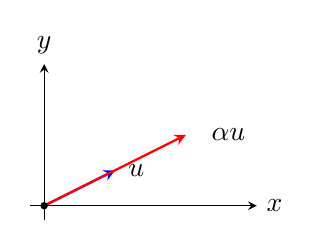
\begin{tikzpicture}[>=stealth,scale=0.9]
            \draw[->] (-0.2,0) -- (3,0) node[right] {$x$};
            \draw[->] (0,-0.2) -- (0,2) node[above] {$y$};
            \draw[->,thick,color=blue] (0,0) -- (1,0.5) ;
            \draw[->,thick,color=red] (0,0) -- (2,1) ;
            \node at (1.3,0.5) {$u$};
            \node at (2.6,1) {$\alpha u$};
            % \node at (1.5,0.2) {$v$};
            \fill (0,0) circle (1.5pt);
        \end{tikzpicture}
    \end{figure}
        
    \end{column}
    \begin{column}{.6\linewidth}
       \begin{block}{Scalar Multiplication}
          For a scalar $\alpha$ (this is a number), the vector $\alpha\mathbf{u}$ stretches or shrinks $\mathbf{u}$ correspondingly. Its direction is along the same line, but its length is scaled by $|\alpha|$. If $\alpha <0$, its direction is reversed.
        \end{block} 
    \end{column}
\end{columns}


  % TODO (diagram): Recreate the collinear arrows labelled u and alpha u.
\end{frame}


\begin{frame}{Vector Arithmetic: Scalar Multiplication}
  % Chinese subtitle in source: 数乘
Let $\mathbf{u}=\begin{bmatrix}1\\2\end{bmatrix}$. Express $\mathbf{u}$, $\mathbf{2u}$, and $\mathbf{\frac{-3}{2}u}$ on a graph.
\only<1>{
    \begin{figure}
    \centering
    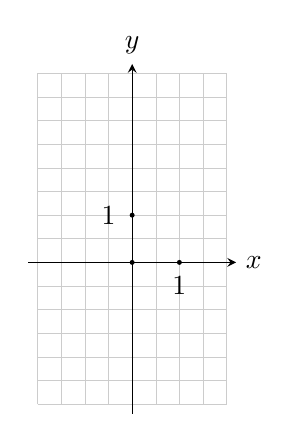
\begin{tikzpicture}[>=stealth,scale=0.6]
    \draw[step=0.5, gray!40, very thin] (-2,-3) grid (2,4);
    \draw[->] (-2.2,0) -- (2.2,0) node[right] {$x$};
    \draw[->] (0,-3.2) -- (0,4.2) node[above] {$y$};
    % \draw[->,thick,color=blue] (0,0) -- (1,2) ;
    % \draw[->,thick,color=red] (0,0) -- (2,4) ;
    % \draw[->,thick,color=brown] (0,0) -- (-1.5,-3) ;
    % \node at (1.3,0.5) {$u$};
    % \node at (2.6,1) {$\alpha u$};
    % \node at (1.5,0.2) {$v$};
    \node at (1,-0.5) {1};
    \node at (-0.5,1) {1};
    \fill (0,0) circle (1.5pt);
    \fill (0,1) circle (1.5pt);
    \fill (1,0) circle (1.5pt);
\end{tikzpicture}
\end{figure}
}
\only<2>{
    \begin{figure}
    \centering
    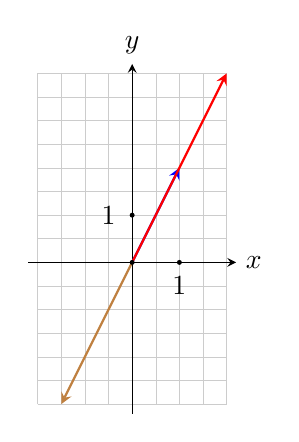
\begin{tikzpicture}[>=stealth,scale=0.6]
    \draw[step=0.5, gray!40, very thin] (-2,-3) grid (2,4);
    \draw[->] (-2.2,0) -- (2.2,0) node[right] {$x$};
    \draw[->] (0,-3.2) -- (0,4.2) node[above] {$y$};
    \draw[->,thick,color=blue] (0,0) -- (1,2) ;
    \draw[->,thick,color=red] (0,0) -- (2,4) ;
    \draw[->,thick,color=brown] (0,0) -- (-1.5,-3) ;
    % \node at (1.3,0.5) {$u$};
    % \node at (2.6,1) {$\alpha u$};
    % \node at (1.5,0.2) {$v$};
    \node at (1,-0.5) {1};
    \node at (-0.5,1) {1};
    \fill (0,0) circle (1.5pt);
    \fill (0,1) circle (1.5pt);
    \fill (1,0) circle (1.5pt);
\end{tikzpicture}
\end{figure}
}
\end{frame}

% ===== Slide 13 =====
\begin{frame}{Vector Addition: recap}
  
    \begin{figure}
        \centering
        $u = \begin{bmatrix}0.5\\2\end{bmatrix}$

        $v = \begin{bmatrix}2\\0.5\end{bmatrix}$

        $u+v = \begin{bmatrix}2+0.5\\2+0.5\end{bmatrix}$
    \end{figure}
\end{frame}

% ===== Slide 14 =====
\begin{frame}{Vector Addition: Geometry and Algebra}
  \begin{center}
    \begin{tabular}{ccc}
        
    Arrows &$\longleftrightarrow$ &Column Matrices\\

    Operations on vectors &$\longleftrightarrow$ &Matrix operations\\
    \end{tabular}
  \end{center}
  \[
    \begin{pmatrix}u_1\\u_2\end{pmatrix}
    +
    \begin{pmatrix}v_1\\v_2\end{pmatrix}
    =
    \begin{pmatrix}u_1+v_1\\u_2+v_2\end{pmatrix}.
  \]
  % TODO (diagram): Add the head-to-tail vector diagram for u+v.
\end{frame}

% ===== Slide 13 =====
\begin{frame}{Scalar Multiplication: recap}
  Let
  \[
    \mathbf{u}=\begin{bmatrix}1\\2\end{bmatrix}.
  \]
  Express $\mathbf{u}$, $2\mathbf{u}$, and
  $-\dfrac{3}{2}\mathbf{u}$ on a graph:
  \[
    \mathbf{u}=\begin{bmatrix}1\\2\end{bmatrix},\qquad
    2\mathbf{u}=\begin{bmatrix}2\\4\end{bmatrix},\qquad
    -\frac32\mathbf{u}=\begin{bmatrix}-\frac32\\-3\end{bmatrix}.
  \]
  % TODO (diagram): Plot all three arrows from the origin on axes
  % x_1 in [-2,2], x_2 in [-3,4].
\end{frame}

% ===== Slide 15 =====
\begin{frame}{Scalar Multiplication: Geometry and Algebra}
  \begin{center}
    \begin{tabular}{ccc}
        Arrows& $\longleftrightarrow$ &Column Matrices\\

    Operations on vectors &$\longleftrightarrow$ &Matrix operations\\

    Geometry& $\dashrightarrow$ &Algebra\\
    \end{tabular}
    
  \end{center}
  \[
    \alpha\begin{pmatrix}u_1\\u_2\end{pmatrix}
    =
    \begin{pmatrix}\alpha u_1\\\alpha u_2\end{pmatrix}.
  \]
  % TODO (diagram): Add the collinear arrows labelled u and alpha u.
\end{frame}

% ===== Slide 16 =====
\begin{frame}{Vector Operations in $\mathbb{R}^2$}
  Let $\mathbf{u},\mathbf{v}\in\mathbb{R}^2$.
  \begin{itemize}
    \item $\mathbf{u}=\mathbf{v}$ if and only if their corresponding entries
          are equal. (exactly equal!)
    \item $\mathbf{u}+\mathbf{v}$ is obtained by adding corresponding entries. 
    \item $c\mathbf{u}$, where $c$ is a scalar, is obtained by multiplying
          each entry in $\mathbf{u}$ by $c$.
  \end{itemize}
  Linear system is defined by solution sets.

  Equality, vector addition, and scalar multiplication in $\mathbb{R}^n$ are defined entry by entry, just as in $\mathbb{R}^2$.
\end{frame}

% ===== Slide 17 =====
\begin{frame}{Eight Algebraic Properties}
  For all $\mathbf{x},\mathbf{y},\mathbf{z}\in\mathbb{R}^n$ and scalars
  $\alpha,\beta$:
  \begin{columns}[T]
    \begin{column}{0.47\textwidth}
      \begin{align*}
        \mathrm{A1}.\;&\mathbf{x}+\mathbf{y}=\mathbf{y}+\mathbf{x}\\
        \mathrm{A2}.\;&(\mathbf{x}+\mathbf{y})+\mathbf{z}
          =\mathbf{x}+(\mathbf{y}+\mathbf{z})\\
        \mathrm{A3}.\;&\mathbf{x}+\mathbf{0}=\mathbf{x}\\
        \mathrm{A4}.\;&\mathbf{x}+(-\mathbf{x})=\mathbf{0}
      \end{align*}
    \end{column}
    \begin{column}{0.53\textwidth}
      \begin{align*}
        \mathrm{A5}.\;&\alpha(\mathbf{x}+\mathbf{y})
          =\alpha\mathbf{x}+\alpha\mathbf{y}\\
        \mathrm{A6}.\;&(\alpha+\beta)\mathbf{x}
          =\alpha\mathbf{x}+\beta\mathbf{x}\\
        \mathrm{A7}.\;&(\alpha\beta)\mathbf{x}
          =\alpha(\beta\mathbf{x})\\
        \mathrm{A8}.\;&1\mathbf{x}=\mathbf{x}
      \end{align*}
    \end{column}
  \end{columns}
\end{frame}

% ===== Slide 18 =====
\begin{frame}{Linear Combinations}
  % Chinese subtitle in source: 线性组合
  Given $\mathbf{v}_1,\ldots,\mathbf{v}_p\in\mathbb{R}^n$ and scalars
  $c_1,\ldots,c_p$, the vector
  \[
    \mathbf{y}=c_1\mathbf{v}_1+c_2\mathbf{v}_2+\cdots+c_p\mathbf{v}_p
  \]
  is called a \alert{linear combination} of
  $\mathbf{v}_1,\ldots,\mathbf{v}_p$, using weights $c_1,\ldots,c_p$.

  Examples include
  \[
    \sqrt{3}\,\mathbf{v}_1+\mathbf{v}_2,\qquad
    \frac12\mathbf{v}_1=\frac12\mathbf{v}_1+0\mathbf{v}_2,\qquad
    \mathbf{0}=0\mathbf{v}_1+0\mathbf{v}_2.
  \]
  The weights may be any real numbers, including zero.
\end{frame}

% ===== Slide 19 =====
\begin{frame}{Example: Linear Combinations in $\mathbb{R}^2$}
  Let
  \[
    \mathbf{v}_1=\begin{bmatrix}2\\1\end{bmatrix},\qquad
    \mathbf{v}_2=\begin{bmatrix}-2\\2\end{bmatrix}.
  \]
  Express each vector as a linear combination of $\mathbf{v}_1$ and
  $\mathbf{v}_2$:
  \[
    \mathbf{a}=\begin{bmatrix}0\\3\end{bmatrix},\quad
    \mathbf{b}=\begin{bmatrix}-4\\1\end{bmatrix},\quad
    \mathbf{c}=\begin{bmatrix}6\\6\end{bmatrix},\quad
    \mathbf{d}=\begin{bmatrix}7\\-4\end{bmatrix}.
  \]
  \begin{figure}
    \centering
    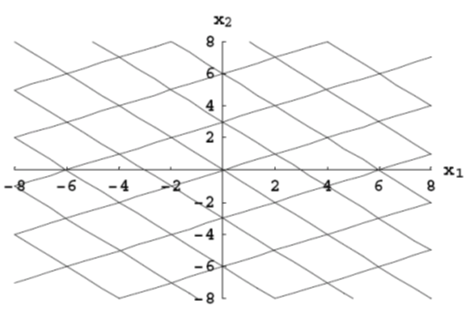
\includegraphics[width=0.3\linewidth]{Lecture2/linearcomb.png}
  \end{figure}
  % TODO (diagram): Recreate the oblique grid generated by v_1 and v_2.
\end{frame}

% ===== Slide 20 =====
\begin{frame}{Example: Solutions}
  \[
    \begin{aligned}
      \mathbf{a}&=\mathbf{v}_1+\mathbf{v}_2, &
      \mathbf{b}&=-\mathbf{v}_1+\mathbf{v}_2,\\
      \mathbf{c}&=4\mathbf{v}_1+\mathbf{v}_2, &
      \mathbf{d}&=\mathbf{v}_1-\frac52\mathbf{v}_2.
    \end{aligned}
  \]
  
  \begin{figure}
    \centering
    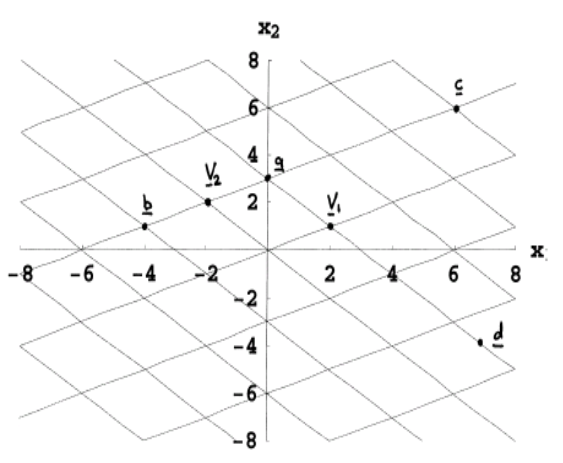
\includegraphics[width=0.3\linewidth]{Lecture2/linearcomb2.png}
  \end{figure}
  % TODO (diagram): Recreate the source grid and label v_1, v_2, a, b, c, d.
\end{frame}

% ===== Slide 21 =====
\begin{frame}{Example: A Vector Equation}
  Let
  \[
    \mathbf{a}_1=\begin{bmatrix}1\\0\\3\end{bmatrix},\quad
    \mathbf{a}_2=\begin{bmatrix}4\\2\\14\end{bmatrix},\quad
    \mathbf{a}_3=\begin{bmatrix}3\\6\\10\end{bmatrix},\quad
    \mathbf{b}=\begin{bmatrix}-1\\8\\-5\end{bmatrix}.
  \]
  Determine whether $\mathbf{b}$ is a linear combination of
  $\mathbf{a}_1,\mathbf{a}_2,\mathbf{a}_3$.

  \medskip
  \pause
  This is equivalent to finding weights $x_1,x_2,x_3$ such that
  \[
    x_1\mathbf{a}_1+x_2\mathbf{a}_2+x_3\mathbf{a}_3=\mathbf{b}.
  \]
\end{frame}

% ===== Slide 22 =====
\begin{frame}{Rewriting the Vector Equation}
    Use the definitions of scalar multiplication and vector addition to rewrite the vector equation:

  \[
    x_1\begin{bmatrix}1\\0\\3\end{bmatrix}
    +x_2\begin{bmatrix}4\\2\\14\end{bmatrix}
    +x_3\begin{bmatrix}3\\6\\10\end{bmatrix}
    =\begin{bmatrix}-1\\8\\-5\end{bmatrix}.
  \]

  \pause

  Which is the same as 

  \[
    \begin{bmatrix}x_1\\0\\3x_1\end{bmatrix}
    +\begin{bmatrix}4x_2\\2x_2\\14x_2\end{bmatrix}
    +\begin{bmatrix}3x_3\\6x_3\\10x_3\end{bmatrix}
    =\begin{bmatrix}-1\\8\\-5\end{bmatrix}.
  \]
\end{frame}

% ===== Slide 23 =====
\begin{frame}{From a Vector Equation to a Linear System}
  \[
    \begin{bmatrix}
      x_1+4x_2+3x_3\\
      2x_2+6x_3\\
      3x_1+14x_2+10x_3
    \end{bmatrix}
    =
    \begin{bmatrix}-1\\8\\-5\end{bmatrix}.
  \]
  By equality of vectors,
  \[
    \begin{cases}
      x_1+4x_2+3x_3=-1,\\
      2x_2+6x_3=8,\\
      3x_1+14x_2+10x_3=-5.
    \end{cases}
  \]
\end{frame}

% ===== Slide 24 =====
\begin{frame}{Solving the Vector Equation}
  The corresponding \textbf{augmented matrix}:
  \[
    \left[\begin{array}{ccc|c}
      1&4&3&-1\\
      0&2&6&8\\
      3&14&10&-5
    \end{array}\right] \pause
    \sim
    \left[\begin{array}{ccc|c}
      1&0&0&1\\
      0&1&0&-2\\
      0&0&1&2
    \end{array}\right].
  \]\pause
  Thus $x_1=1$, $x_2=-2$, and $x_3=2$. Therefore $\mathbf{b}$ is a linear combination of $\mathbf{a_1}$, $\mathbf{a_2}$, and $\mathbf{a_3}$.

  \[
    \mathbf{b}=\mathbf{a}_1-2\mathbf{a}_2+2\mathbf{a}_3.
  \]
\end{frame}

% ===== Slide 25 =====
\begin{frame}{Vector Equations and Augmented Matrices}
  A solution of
  \[
    x_1\mathbf{a}_1+x_2\mathbf{a}_2+x_3\mathbf{a}_3=\mathbf{b}
  \]
  is found by solving the linear system whose augmented matrix is
  \[
    \begin{bmatrix}\mathbf{a}_1&\mathbf{a}_2&\mathbf{a}_3&\mathbf{b}\end{bmatrix}.
  \]

  Review of the last example: $\mathbf{a}_1,\mathbf{a}_2,\mathbf{a}_3$ and $\mathbf{b}$ are columns of the augmented matrix.
  \[
    \left[\begin{array}{ccc|c}
      1&4&3&-1\\
      0&2&6&8\\
      3&14&10&-5
    \end{array}\right].
  \]
  \begin{figure}
    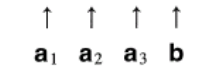
\includegraphics[width=.25\linewidth]{Lecture2/snippet1.png}
\end{figure}
\end{frame}



% ===== Slide 26 =====
\begin{frame}{Vector Equation and Linear System}
  The vector equation
  \[
    x_1\mathbf{a}_1+x_2\mathbf{a}_2+\cdots+x_n\mathbf{a}_n=\mathbf{b}
  \]
  has the same solution set as the linear system whose augmented matrix is
  \[
    \begin{bmatrix}\mathbf{a}_1&\mathbf{a}_2&\cdots&\mathbf{a}_n&\mathbf{b}\end{bmatrix}.
  \]
  In particular, $\mathbf{b}$ can be generated by a linear combination of
  $\mathbf{a}_1,\ldots,\mathbf{a}_n$ if and only if the corresponding
  linear system is consistent.
\end{frame}

% ===== Slide 27 =====
\begin{frame}{Vector Equations and Ordinary Systems}
  \begin{center}
    \Large Vector equations $\Longleftrightarrow$ Ordinary systems of equations
  \end{center}

  \medskip

  \textbf{The key idea of linear algebra} is to find a solution\pause

  The solution here is to find all \textbf{vectors} satisfying the system...\pause

  ... that are written as a linear combination of a fixed set
  $\{\mathbf{v}_1,\ldots,\mathbf{v}_p\}$ of vectors.
\end{frame}

% ===== Slide 28 =====
\begin{frame}{Span $\{\mathbf{v}_1,\ldots,\mathbf{v}_p\}$}
  If $\mathbf{v}_1,\ldots,\mathbf{v}_p\in\mathbb{R}^n$, then the set of all
  their linear combinations is denoted by
  \[
    \operatorname{Span}\{\mathbf{v}_1,\ldots,\mathbf{v}_p\}.
  \]
  It is the subset of $\mathbb{R}^n$ \alert{spanned} (or \alert{generated})
  by $\mathbf{v}_1,\ldots,\mathbf{v}_p$; that is, the collection of all
  vectors of the form
  \[
    c_1\mathbf{v}_1+c_2\mathbf{v}_2+\cdots+c_p\mathbf{v}_p,
  \]

 \qquad $c_1,\ldots,c_p$ being scalars.
\end{frame}

\begin{frame}{Span}
    Span is not "a" vector. It tells us what shapes of vectors can be generated:
    \begin{figure}
            \centering
            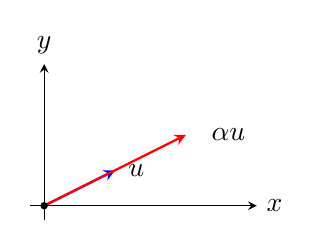
\begin{tikzpicture}[>=stealth,scale=0.9]
            \draw[->] (-0.2,0) -- (3,0) node[right] {$x$};
            \draw[->] (0,-0.2) -- (0,2) node[above] {$y$};
            \draw[->,thick,color=blue] (0,0) -- (1,0.5) ;
            \draw[->,thick,color=red] (0,0) -- (2,1) ;
            \node at (1.3,0.5) {$u$};
            \node at (2.6,1) {$\alpha u$};
            % \node at (1.5,0.2) {$v$};
            \fill (0,0) circle (1.5pt);
        \end{tikzpicture}
    \end{figure}
        
    This only has one direction.
\end{frame}


\begin{frame}{Span}
    How to use the minimal amount of vectors to span the entire plane?
    \begin{figure}
            \centering
            \begin{tikzpicture}[>=stealth,scale=0.9]
            \draw[->] (-0.2,0) -- (3,0) node[right] {$x$};
            \draw[->] (0,-0.2) -- (0,3) node[above] {$y$};
            \draw[->,thick,color=blue] (0,0) -- (0,2) ;
            \draw[->,thick,color=red] (0,0) -- (2,0) ;
            \node at (-0.5,1.5) {$y$};
            \node at (1.5,-0.5) {$x$};
            \fill (0,0) circle (1.5pt);
        \end{tikzpicture}
    \end{figure}
    Combining $\mathbf{x}$ and $\mathbf{y}$ we can reach any point in the plane.
    \[
\operatorname{span}\left\{
\begin{bmatrix}
1\\
0
\end{bmatrix},
\begin{bmatrix}
0\\
1
\end{bmatrix}
\right\}
=
\mathbb{R}^2.
\]
\end{frame}


% ===== Slide 29 =====
\begin{frame}{A Geometric Description of $\operatorname{Span}\{\mathbf{v}\}$}
  Let $\mathbf{v}$ be a nonzero vector in $\mathbb{R}^3$. Then
  $\operatorname{Span}\{\mathbf{v}\}$ is the set of all scalar multiples
  of $\mathbf{v}$, namely the line in $\mathbb{R}^3$ through
  $\mathbf{v}$ and $\mathbf{0}$.

\begin{figure}
    \centering
    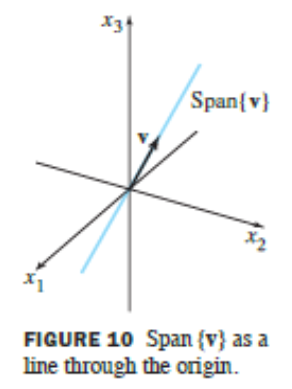
\includegraphics[width=0.3\linewidth]{Lecture2/span3.png}
\end{figure}
  % TODO (diagram): Draw 3-D axes and the line through the origin in direction v.
\end{frame}

% ===== Slide 30 =====
\begin{frame}{A Geometric Description of $\operatorname{Span}\{\mathbf{u},\mathbf{v}\}$}
  \begin{itemize}
    \item If $\mathbf{u}$ and $\mathbf{v}$ are nonzero vectors in
          $\mathbb{R}^3$, with $\mathbf{v}$ \textbf{not a scalar multiple} of
          $\mathbf{u}$, then $\operatorname{Span}\{\mathbf{u},\mathbf{v}\}$
          is the plane in $\mathbb{R}^3$ containing
          $\mathbf{u}$, $\mathbf{v}$, and $\mathbf{0}$.
    \item In particular, Span \{$\mathbf{u},\mathbf{v}$\} contains the line $\mathbb{R}^3$ through
          $\mathbf{u}$ and $\mathbf{0}$ and the line through
          $\mathbf{v}$ and $\mathbf{0}$.
  \end{itemize}
  % TODO (diagram): Draw the plane generated by u and v, with sample multiples.
  \begin{figure}
    \centering
    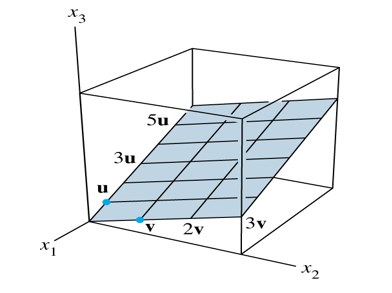
\includegraphics[width=.4\linewidth]{Lecture2/fig11.png}
  \end{figure}
\end{frame}

% ===== Slide 31 =====
\begin{frame}{Example: Is $\mathbf{b}$ in the Span?}
  Let
  \[
    \mathbf{a}_1=\begin{bmatrix}1\\-2\\3\end{bmatrix},\quad
    \mathbf{a}_2=\begin{bmatrix}5\\-13\\-3\end{bmatrix},\quad
    \mathbf{b}=\begin{bmatrix}-3\\8\\1\end{bmatrix}.
  \]
  Is $\mathbf{b}$ in $\operatorname{Span}\{\mathbf{a}_1,\mathbf{a}_2\}$?
  \[
    \left[\begin{array}{cc|c}1&5&-3\\-2&-13&8\\3&-3&1\end{array}\right]
    \sim
    \left[\begin{array}{cc|c}1&5&-3\\0&-3&2\\0&-18&10\end{array}\right]
    \sim
    \left[\begin{array}{cc|c}1&5&-3\\0&-3&2\\0&0&-2\end{array}\right].
  \]
  The third equation is $0=-2$, so the system has no solution. Hence
  $\mathbf{b}\notin\operatorname{Span}\{\mathbf{a}_1,\mathbf{a}_2\}$.
\end{frame}
